\setcounter{dang}{0}% \newpage
% \begin{name}
% 	{GV biên soạn: Thien Tran Xuan\\ GV phản biện 1: Huynh Quy\\ GV phản biện 2: Đỗ Tấn Lộc}
% 	{TOÁN 10-KNTT-CS}
% \end{name}
\setcounter{section}{2}
\section{Dấu của tam thức bậc hai}
\subsection{KIẾN THỨC TRỌNG TÂM}
\subsubsection{Dấu của tam thức bậc hai}
\begin{dn}
	Tam thức bậc hai (đối với $x$ ) là biểu thức có dạng $f(x)=ax^2+bx+c$. Trong đó $a$, $b$, $c$ là những số cho trước với $a\ne 0$.
\end{dn}
\begin{note}
	\begin{itemize}
		\item Nghiệm của phương trình $ax^2+bx+c=0$ được gọi là nghiệm của tam thức bậc hai.
		\item $ \Delta =b^2-4ac$ và $ \Delta '=b'^2-ac$ theo thứ tự được gọi là biệt thức và biệt thức thu gọn của tam thức bậc hai.
	\end{itemize}
\end{note}

\iconMT~ Ta đã biết hàm số $y=ax^2+bx+c$ với $a \ne 0$ có đồ thị là một parabol.
\begin{center}
	\begin{tabular}{|c|c|c|c|}
		\hline
		& $\Delta <0$ 
		& $\Delta =0$ 
		& $\Delta >0$ \\
		\hline
		$a>0$ 
		& 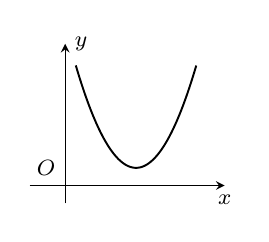
\begin{tikzpicture}[smooth,samples=300,scale=0.45,>=stealth,font=\footnotesize]
				\draw[->] (-1,0)--(4.5,0) node[below]{$x$};
				\draw[->] (0,-0.5)--(0,4) node[right]{$y$};
				\draw (0,0) node[above left]{$O$};
				\draw[line width=0.7pt,domain=0.3:3.7] plot(\x,{(\x)^2-4*(\x)+4.5});
				% \node[below] at (2,4) {\fbox{\scriptsize$\Delta <0$}};
			\end{tikzpicture}
		& \begin{tikzpicture}[smooth,samples=300,scale=0.45,>=stealth,font=\footnotesize]
				\draw[->] (-1,0)--(4.5,0) node[below]{$x$};
				\draw[->] (0,-0.5)--(0,3.5) node[left]{$y$};
				\draw (0,0) node[above left]{$O$};
				\draw[line width=0.7pt,domain=0.3:3.7] plot(\x,{(\x)^2-4*(\x)+4});
				\draw[fill=black] (2,0) circle(1.5pt);
				\node[below] at (2,0) {$-\dfrac{b}{2a}$};
				% \node[below] at (2,3.8) {\fbox{\scriptsize$\Delta =0$}};
			\end{tikzpicture}
		& 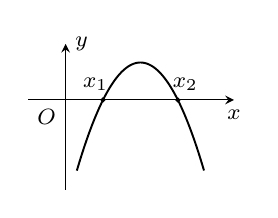
\begin{tikzpicture}[smooth,samples=300,scale=0.475,>=stealth,font=\footnotesize]
				\draw[->] (-1,0)--(4.5,0) node[below]{$x$};
				\draw[->] (0,-2.4)--(0,1.5) node[right]{$y$};
				\draw (0,0) node[below left]{$O$};
				\draw[line width=0.7pt,domain=0.3:3.7] plot(\x,{-(\x)^2+4*(\x)-3});
				\draw[fill=black] (1,0) circle(1.5pt) (3,0) circle(1.5pt);
				\node[above] at (0.8,0) {$x_1$};
				\node[above] at (3.2,0) {$x_2$};
				% \node[below] at (2,-1.5) {\fbox{\scriptsize$\Delta >0$}};
			\end{tikzpicture}\\
			\hline
		$a<0$
		& 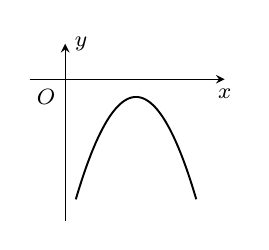
\begin{tikzpicture}[smooth,samples=300,scale=0.45,>=stealth,font=\footnotesize]
				\draw[->] (-1,0)--(4.5,0) node[below]{$x$};
				\draw[->] (0,-4)--(0,1) node[right]{$y$};
				\draw (0,0) node[below left]{$O$};
				\draw[line width=0.7pt,domain=0.3:3.7] plot(\x,{-(\x)^2+4*(\x)-4.5});
				% \node[below] at (2,-2) {\fbox{\scriptsize$\Delta <0$}};
			\end{tikzpicture}
		& \begin{tikzpicture}[smooth,samples=300,scale=0.45,>=stealth,font=\footnotesize]
				\draw[->] (-1,0)--(4.5,0) node[below]{$x$};
				\draw[->] (0,-3.5)--(0,1) node[left]{$y$};
				\draw (0,0) node[below left]{$O$};
				\draw[line width=0.7pt,domain=0.3:3.7] plot(\x,{-(\x)^2+4*(\x)-4});
				\draw[fill=black] (2,0) circle(1.5pt);
				\node[above] at (2,0) {$-\dfrac{b}{2a}$};
				% \node[below] at (2,-2) {\fbox{\scriptsize$\Delta =0$}};
			\end{tikzpicture}
		& 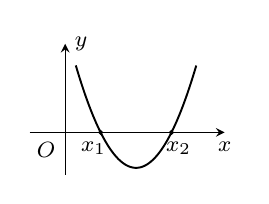
\begin{tikzpicture}[smooth,samples=300,scale=0.45,>=stealth,font=\footnotesize]
				\draw[->] (-1,0)--(4.5,0) node[below]{$x$};
				\draw[->] (0,-1.2)--(0,2.5) node[right]{$y$};
				\draw (0,0) node[below left]{$O$};
				\draw[line width=0.7pt,domain=0.3:3.7] plot(\x,{(\x)^2-4*(\x)+3});
				\draw[fill=black] (1,0) circle(1.5pt) (3,0) circle(1.5pt);
				\node[below] at (0.8,0) {$x_1$};
				\node[below] at (3.2,0) {$x_2$};
				% \node[below] at (2,2.5) {\fbox{\scriptsize$\Delta >0$}};
			\end{tikzpicture}\\
			\hline
	\end{tabular}
\end{center}
% \textbf{\iconMT~ Tương ứng hình ảnh đồ thị ở trên, ta có bảng tổng kết dấu của tam thức bậc hai như sau:}
% \begin{itemize}
% 	\item Nếu $a>0$:
% 	\begin{listEX}[3]
% 		\item [] \begin{tikzpicture}[scale=0.8,font=\footnotesize]
% 			\tkzTabInit[nocadre=false,lgt=1,espcl=2.5]
% 			{$x$ /0.6,$f(x)$ /0.6}
% 			{$-\infty$,$+\infty$}
% 			\tkzTabLine{,+,}
% 		\end{tikzpicture}
% 		\item [] \begin{tikzpicture}[scale=0.8,font=\footnotesize]
% 			\tkzTabInit[nocadre=false,lgt=1,espcl=1.4]
% 			{$x$ /0.6,$f(x)$ /0.6}
% 			{$-\infty$,$x_0$,$+\infty$}
% 			\tkzTabLine{,+,$0$,+,}
% 		\end{tikzpicture}
% 		\item [] \begin{tikzpicture}[scale=0.8,font=\footnotesize]
% 			\tkzTabInit[nocadre=false,lgt=1,espcl=1.2]
% 			{$x$ /0.6,$f(x)$ /0.6}
% 			{$-\infty$,$x_1$,$x_2$,$+\infty$}
% 			\tkzTabLine{,+,$0$,-,$0$,+,}
% 		\end{tikzpicture}
% 	\end{listEX}
% 	\item Nếu $a<0$:
% 	\begin{listEX}[3]
% 		\item [] \begin{tikzpicture}[scale=0.8,font=\footnotesize]
% 			\tkzTabInit[nocadre=false,lgt=1,espcl=2.5]
% 			{$x$ /0.6,$f(x)$ /0.6}
% 			{$-\infty$,$+\infty$}
% 			\tkzTabLine{,-,}
% 		\end{tikzpicture}
% 		\item [] \begin{tikzpicture}[scale=0.8,font=\footnotesize]
% 			\tkzTabInit[nocadre=false,lgt=1,espcl=1.4]
% 			{$x$ /0.6,$f(x)$ /0.6}
% 			{$-\infty$,$x_0$,$+\infty$}
% 			\tkzTabLine{,-,$0$,-,}
% 		\end{tikzpicture}
% 		\item [] \begin{tikzpicture}[scale=0.8,font=\footnotesize]
% 			\tkzTabInit[nocadre=false,lgt=1,espcl=1.2]
% 			{$x$ /0.6,$f(x)$ /0.6}
% 			{$-\infty$,$x_1$,$x_2$,$+\infty$}
% 			\tkzTabLine{,-,$0$,+,$0$,-,}
% 		\end{tikzpicture}
% 	\end{listEX}
% \end{itemize}
\begin{dl}[Định lý về dấu tam thức bậc hai]
	Cho tam thức bậc hai $f(x)=ax^2+b x+c\,(a \neq 0)$.
	\begin{itemize}
		\item Nếu $\Delta<0$ thì $f(x)$ cùng dấu với hệ số $a$ với mọi $x \in \mathbb{R}$.
		\item Nếu $\Delta=0$ thì $f(x)$ cùng dấu với hệ số $a$ với mọi $x \neq-\frac{b}{2 a}$.
		\item Nếu $\Delta>0$ thì tam thức $f(x)$ có hai nghiệm phân biệt $x_1$ và $x_2$ $\left(x_{1}<x_{2}\right)$. Khi đó, $f(x)$ cùng dấu với hệ số $a$ với mọi $x \in\left(-\infty ; x_{1}\right) \cup\left(x_{2} ;+\infty\right) ; f(x)$ trái dấu với hệ số $a$ với mọi $x \in\left(x_{1} ; x_{2}\right)$
	\end{itemize}
\end{dl}

\begin{boxdn}
	\textbf{Ghi nhớ dấu của $f(x)$ và $a$}
	\begin{itemize}
		\item Nếu $\Delta < 0$ thì\\
		\begin{tikzpicture}
			\tkzTabInit[nocadre=false,lgt=1.5,espcl=4.2]
			{$x$ /0.7,$f(x)$ /0.8}
			{$-\infty$,$+\infty$}
			\tkzTabLine{,\text{cùng dấu },}
		\end{tikzpicture}
		\item Nếu $\Delta = 0$ thì\\
		\begin{tikzpicture}
			\tkzTabInit[nocadre=false,lgt=1.2,espcl=2.5]
			{$x$ /1,$f(x)$ /0.8}
			{$-\infty$,$-\frac{b}{2a}$,$+\infty$}
			\tkzTabLine{,\text{cùng dấu },$0$,\text{ cùng dấu },}
		\end{tikzpicture}
		\item Nếu $\Delta > 0$ thì\\
		\begin{tikzpicture}
			\tkzTabInit[nocadre=false,lgt=1.2,espcl=3]
			{$x$ /0.7,$f(x)$ /1}
			{$-\infty$,$x_1$,$x_2$,$+\infty$}
			\tkzTabLine{,\text{cùng dấu },$0$,\text{ trái dấu },$0$,\text{ cùng dấu },}
		\end{tikzpicture}
	\end{itemize}
\end{boxdn}

\subsubsection{Bất phương trình bậc hai}
\begin{dn}
	Bất phương trình bậc hai ẩn $x$ là bất phương trình có dạng $a x^{2}+b x+c>0$ (hoặc $\left.ax^2 + bx + c \geq 0, ax^2 + bx+c<0, a x^{2}+b x+c \leq 0\right)$, trong đó $a, b, c$ là những số thực đã cho và $a \neq 0$.
\end{dn}
\begin{boxdn}
	Cho tam thức bậc hai $ax^2+bx+c$, với $a \ne 0$.
	\begin{multicols}{2}
		\begin{enumerate}
			\item $ax^2+bx+c>0, \forall x\in \mathbb{R} \Leftrightarrow \heva{&a>0\\& \Delta <0.}$
			\item $ax^2+bx+c<0, \forall x \in \mathbb{R} \Leftrightarrow \heva{&a<0\\& \Delta <0.}$
			\item $ax^2+bx+c \geq 0, \forall x\in \mathbb{R} \Leftrightarrow \heva{&a>0\\
				& \Delta \leq 0.}$
			\item $ax^2+bx+c \leq 0, \forall x\in \mathbb{R} \Leftrightarrow \heva{&a<0\\ & \Delta \leq 0.}$
		\end{enumerate}
	\end{multicols}
\end{boxdn}

\subsection{PHÂN LOẠI VÀ PHƯƠNG PHÁP GIẢI TOÁN}
\begin{dang}{Xét dấu tam thức bậc hai $f(x)=ax^2+bx+c$, với $a \ne 0$.}
	\begin{itemize}
		\item [$\bullet$] Tìm nghiệm $ax^2+bx+c=0 \quad (1)$.
		\item [$\bullet$] Tùy thuộc vào số nghiệm của (1), ta lựa chọn bảng xét dấu phù hợp.
	\end{itemize}
	\begin{note}
		Ghi nhớ ngắn gọn: Nếu $\Delta \le 0$ thì cùng dấu $a$; Nếu $\Delta >0 $ thì  "trong trái, ngoài cùng".
	\end{note}
\end{dang}
\begin{vd}%[0D4Y5-1]
	Xét dấu của các tam thức sau
	\begin{listEX}[1]
		\item $3x^2-2x+1$.
		\item $-x^2+4x+5$.
		\item $4x^2+4x+1$.
		\item $2x^2 - 6x + 4{,}5$.
		\item $3x^2 - 2x - 8$ .
		\item $- x^2 + 2x - 1$.
	\end{listEX}
	\loigiai{
		\begin{listEX}
			\item Ta có $ \Delta '=-2<0$ và $a=3>0$. Suy ra $3x^2-2x+1>0,\forall x\in \mathbb{R}$.
			\item Ta có $-x^2+4x+5=0 \Leftrightarrow \left[\begin{aligned}& x=-1 \\ & x=5.\end{aligned}\right. $\\
			Bảng xét dấu
			\begin{center}
				
\begin{tikzpicture}
					\tkzTabInit[lgt=3,espcl=2]
					{$x$ /0.8, $-x^2+4x+5$ /0.8}
					{$-\infty$,$-1$,$5$,$+\infty$}
					\tkzTabLine{ ,-,$0$,+,$0$,-,}
				\end{tikzpicture}
			\end{center}
			Suy ra $-x^2+4x+5>0 \Leftrightarrow x\in (-1;5)$ và $-x^2+4x+5<0 \Leftrightarrow x\in (-\infty;-1)\cup (5;+\infty)$.
			\item Tam thức bậc hai $f(x)=4x^2+4x+1$ có $\Delta=0$, nghiệm kép $x_0=-\dfrac{1}{2}$ và hệ số $a=4>0$ nên $f(x)>0$ với mọi $x\in\mathbb{R}\setminus\left\{-\dfrac{1}{2}\right\}$.
			\item Ta có $f(x)=0 \Leftrightarrow 2x^2-6x+\dfrac{9}{2}=0 \Leftrightarrow x=\dfrac{3}{2}$.\\ 
			Bảng xét dấu
			\begin{center}
				
\begin{tikzpicture}
					\tkzTabInit[nocadre=false,lgt=1.2,espcl=4,deltacl=0.6] %phần bắt buộc
					{$x$ /1,$f(x)$ /0.6}
					{$-\infty$,$\dfrac{3}{2}$,$+\infty$}
					\tkzTabLine{,+,$0$,+,}
				\end{tikzpicture}
			\end{center}
			Vậy $f(x) > 0, \forall x \ne \dfrac{3}{2}$.
			\item Ta có $f(x)=0\Leftrightarrow 3x^2-2x-8=0 \Leftrightarrow \hoac{& x=-\dfrac{4}{3} \\ & x=2}$.\\ 
			Bảng xét dấu
			\begin{center}
				
\begin{tikzpicture}
					\tkzTabInit[nocadre=false,lgt=1.2,espcl=2.5,deltacl=0.6] %phần bắt buộc
					{$x$ /1,$f(x)$ /0.6}
					{$-\infty$,$-\dfrac{4}{3}$,$2$,$+\infty$}
					\tkzTabLine{,+,$0$,-,$0$,+,}
				\end{tikzpicture}
			\end{center}
			Vậy $f(x) > 0 \Leftrightarrow x \in \left(-\infty; -\dfrac{4}{3}\right) \cup (2; +\infty)$; $f(x) < 0 \Leftrightarrow x \in \left(-\dfrac{4}{3}; 2\right)$.
			\item Ta có $f(x)=0 \Leftrightarrow -x^2+2x-1=0\Leftrightarrow x=1$.\\ Bảng xét dấu
			\begin{center}
				
\begin{tikzpicture}
					\tkzTabInit[nocadre=false,lgt=1.2,espcl=4,deltacl=0.6] %phần bắt buộc
					{$x$ /1,$f(x)$ /0.6}
					{$-\infty$,$1$,$+\infty$}
					\tkzTabLine{,-,$0$,-,}
				\end{tikzpicture}
			\end{center}
			Vậy $f(x) < 0, \forall x \ne 1$.
		\end{listEX}
	}
\end{vd}

\begin{dang}{Giải bất phương trình bậc hai $ax^2+bx+c \ge 0$, với $a \ne 0$}
	\begin{itemize}
		\item [$\bullet$] Đặt $f(x) = ax^2+bx+c=0 \quad (1)$.
		\item [$\bullet$] Xét dấu $f(x)$.
		\item [$\bullet$] Dựa vào bảng xét dấu đưa ra kết luận về nghiệm của bất phương trình $f(x) \ge 0$.
	\end{itemize}
\end{dang}
\begin{vd}%[0D4Y5-2]
	Giải các bất phương trình sau	
	\begin{listEX}[1]
		\item $-3x^2+2x+1<0$.
		\item $x^2+x-12\ge 0$.
		\item $-x^2+x+6 \le 0$.
		\item $-x^2+x-5<0$
		\item $x^2-2x-4>0$
		\item $4x^2+4x+1>0$
	\end{listEX}
	\loigiai{
		\begin{listEX}
			\item Ta có $-3x^2+2x+1=0 \Leftrightarrow x=-\dfrac{1}{3}$ hoặc $x=1$.\\
			Bảng xét dấu
			\begin{center}
				
\begin{tikzpicture}
					\tkzTabInit[lgt=3,espcl=2]
					{$x$ /1.2, $-x^2+4x+5$ /0.8}
					{$-\infty$,$-\dfrac{1}{3}$,$1$,$+\infty$}
					\tkzTabLine{ ,-,$0$,+,$0$,-,}
				\end{tikzpicture}
			\end{center}
			Dựa vào bảng xét dấu, ta có tập nghiệm của bất phương trình là $S=\left(-\infty;-\dfrac{1}{3}\right)\cup (1;+\infty)$.
			\item Ta có $x^2+x-12=0 \Leftrightarrow x=3$ hoặc $x=-4$.\\
			Bảng xét dấu
			\begin{center}
				
\begin{tikzpicture}
					\tkzTabInit[lgt=3,espcl=2]
					{$x$ /0.8, $x^2+x-12$/0.8}
					{$-\infty$,$-4$,$3$,$+\infty$}
					\tkzTabLine{ ,+,$0$,-,$0$,+,}
				\end{tikzpicture}
			\end{center}
			Dựa vào bảng xét dấu, ta có tập nghiệm của bất phương trình là $S=(-\infty;-4] \cup [3;+\infty)$.	
			\item Ta có $-x^2+x+6=0 \Leftrightarrow x=-2$ hoặc $x=3$.\\
			Bảng xét dấu
			\begin{center}
				
\begin{tikzpicture}
					\tkzTabInit[lgt=3,espcl=2]
					{$x$ /1.2, $-x^2+x+6$ /0.8}
					{$-\infty$,$-2$,$3$,$+\infty$}
					\tkzTabLine{ ,-,$0$,+,$0$,-,}
				\end{tikzpicture}
			\end{center}
			Dựa vào bảng xét dấu, ta có tập nghiệm của bất phương trình là $S=\left(-\infty;-2\right]\cup [3;+\infty)$.
			\item $-x^2+x-5=0$ vô nghiệm nên ta có bảng xét dấu
			\begin{center}
				
\begin{tikzpicture}
					\tkzTabInit[lgt=3,espcl=2]
					{$x$ /0.8, $-x^2+x-5$ /0.8}
					{$-\infty$,$+\infty$}
					\tkzTabLine{ ,-,}
				\end{tikzpicture}
			\end{center}
			Dựa vào bảng xét dấu, ta có tập nghiệm của bất phương trình là $\mathbb{R}$.
			\item Ta có $4x^2+4x+1=0\Leftrightarrow x=-\dfrac{1}{2} $.\\
			Bảng xét dấu
			\begin{center}
				
\begin{tikzpicture}
					\tkzTabInit[lgt=3,espcl=2]
					{$x$ /1.2, $4x^2+4x+1$ /0.8}
					{$-\infty$,$-\frac{1}{2}$,$+\infty$}
					\tkzTabLine{ ,+,$0$,+,}
				\end{tikzpicture}
			\end{center}
			Tập nghiệm của bất phương trình là $\mathbb{R}\setminus\left\{-\dfrac{1}{2}\right\}$.
			
		\end{listEX}
	}
\end{vd}

\begin{dang}{Bài toán tham số.}
	\begin{itemize}
		\item [$\bullet$] Dựa vào yêu cầu đề bài để đưa ra điều kiện tương đương.
		\item [$\bullet$] Áp dụng giải bất phương trình bậc hai để tìm giá trị của tham số $m$.
	\end{itemize}
\end{dang}

\begin{vd}%[0D7H2-6]
	Tìm các giá trị của tham số $m$ để 
	\begin{enumEX}[a)]{1}
		\item $x^2 - 2x + m \geq 0,\, \forall x\in  \mathbb{R}$.
		\item $x^2 -2mx + 4- 3m>0,\, \forall x\in  \mathbb{R} $. 
		\item $-x^2 -2 (2m-1) x+ 1 -2m \le 0,\, \forall x\in  \mathbb{R} $. 
		\item $-2x^2+2(m-2)x+m-2<0,\, \forall x\in  \mathbb{R} $. 
	\end{enumEX}
	\loigiai{
		\begin{itemize}
			\item [a)] Bất phương trình thỏa mãn với mọi số thực thì $\Delta \leq 0 \ (\Delta' \leq 0)$.\\
			$\Delta' = (-1)^2 - m \leq 0 \Leftrightarrow m \geq 1$.
			\item [b)] Ta có $\Delta '= b'^2 -a c = m^2 + 3m-4$.\\
			Khi đó $P(x) >0 $ $\forall x \Leftrightarrow \heva{& a > 0\\& \Delta ' <0 } \Leftrightarrow \heva{& 1 >0 \text{ (luôn đúng)}\\& m^2 + 3m -4 < 0} \Leftrightarrow m^2 + 3m -4 <0$.\\
			Bảng xét dấu \\
			\begin{center}
				
\begin{tikzpicture}
					\tkzTabInit
					[lgt=2.5,espcl=2] % tùy chọn
					{$m $/1, $m^2 + 3m -4 $/1.3} % cột 1
					{$-\infty $,$-4$,$1$,$+ \infty $} % hàng 1 cột 2
					\tkzTabLine{, +  , z , - , z , + , } % hàng 2 cột 2
				\end{tikzpicture}
			\end{center}
			Dựa vào bảng xét dấu ta thấy $m \in (-4;1)$ thoả mãn yêu cầu bài toán.
			\item [c)] Ta có $\Delta ' = b'^2 - ac = (2m-1)^2 + (1-2m) = 4m^2 -6m +2. $\\
			Khi đó $P(x) \le 0$ $\forall x \Leftrightarrow \heva{&a <0 \\& \Delta ' \le 0} \Leftrightarrow \heva{&-1<0 \text{ (luôn đúng)} \\& 4m^2 - 6m+2 \le 0} \Leftrightarrow 4m^2 - 6m+2 \le 0. $\\
			Bảng xét dấu \\
			\begin{center}
				
\begin{tikzpicture}
					\tkzTabInit
					[lgt=3 ,espcl=2] % tùy chọn
					{$m$/1, $4m^2 -6m +2  $/1.3} % cột 1
					{$-\infty $,$\dfrac{1}{2}$,$1$,$+ \infty $} % hàng 1 cột 2
					\tkzTabLine{, +  , z , - , z , + , } % hàng 2 cột 2
				\end{tikzpicture}
			\end{center}
			Dựa vào bảng xét dấu ta thấy $m \in \left[ \dfrac{1}{2};1\right]$ thoả mãn yêu cầu bài toán.
			\item [d)] Yêu cầu bài toán tương đương với
			{\allowdisplaybreaks
				\begin{eqnarray*}
					&&f(x)=-2x^2+2(m-2)x+m-2\le 0,\forall x\in\mathbb{R} \\
					&\Leftrightarrow & \Delta' =(m-2)^2+2\cdot(m-2)< 0\\
					&\Leftrightarrow & m(m-2)< 0\\
					&\Leftrightarrow & 0< m< 2.
			\end{eqnarray*}}
			Vậy, giá trị cần tìm của $m$ là $0< m< 2$.
		\end{itemize}
	}
\end{vd}

\begin{dang}{Bài toán thực tế.}
	\begin{itemize}
		\item [$\bullet$] Chuyển ngôn ngữ bài toán thực tế về bài toán bất phương trình.
		\item [$\bullet$] Áp dụng cách giải bất phương trình.
	\end{itemize}
\end{dang}
\begin{vd}%[0D7H2-7]
	Độ cao so với mặt đất của một quả bóng được ném lên theo phương thẳng đứng được mô tả bởi hàm số bậc hai $h(t)=-4,9 t^{2}+20 t+1$, ở đó độ cao $h(t)$ tính bằng mét và thời gian $t$ tính bằng giây. Trong khoảng thời điểm nào trong quá trình bay của nó, quả bóng sẽ ở độ cao trên $5$ m so với mặt đất?
	\loigiai{
		Xét bất phương trình $$-4,9 t^{2}+20 t+1>5\Leftrightarrow-4,9 t^{2}+20 t-4>0.$$
		Nghiệm của phương trình $-4,9 t^{2}+20 t-4=0$ là $t \approx 0,21 ; t \approx 3,87$.\\
		Do đó, nghiệm của bất phương trình là $t \in(0,21 ; 3,87)$.\\
		Vậy khoảng thời điểm $t \in(0,21 ; 3,87)$ (s) trong quá trình bay của quả bóng thì nó sẽ ở độ cao trên $5 \mathrm{~m}$ so với mặt đất.
	}
\end{vd}

\begin{vd}%[0D7H2-7]
	Một vật được ném theo phương thẳng đứng xuống dưới từ độ cao $320 \mathrm{~m}$ với vận tốc ban đầu $v_{Q}=20 \mathrm{~m} / \mathrm{s}$. Hỏi sau ít nhất bao nhiêu giây, vật đó cách mặt đất không quá $100 \mathrm{~m}$ ? Giả thiết rằng sức cản của không khí là không đáng kể.
	\loigiai{
		Độ cao của vật so với mặt đất được cho bởi công thức
		$$
		h(t)=h_{0}+v_{0} t-\frac{1}{2} g t^{2}=320+20 t-4,9 t^{2}(\mathrm{~m}) .
		$$
		Vật cách mặt đất không quá $100 \mathrm{~m}$ khi và chỉ khi $h(t) \leq 100$, tức là $-4,9 t^{2}+20 t+320 \leq 100$ hay tương đương $4,9 t^{2}-20 t-220 \geq 0$.\\
		Giải bất phương trình này và chú ý đến điều kiện $t>0$ ta được: $t \geq \frac{10+\sqrt{1178}}{4,9} \approx 9,05(\mathrm{~s})$.
	}
\end{vd}

\begin{vd}%[0D7V2-7]
	\immini{Xét đường tròn đường kính $AB=4$ và một điểm $M$ di chuyển trên đoạn $A B$, đặt $A M=x$. Xét hai đường tròn đường kính $A M$ và $M B$. Kí hiệu $S(x)$ là diện tích phần hình phẳng nằm trong hình tròn lớn và nằm ngoài hai hình tròn nhỏ. Xác định các giá trị của $x$ để diện tích $S(x)$ không vượt quá một nửa tổng diện tích hai hình tròn nhỏ.}{
		\begin{tikzpicture}[smooth,font=\footnotesize,scale=1,>=latex]
			\path
			(0,0) coordinate (A)
			(4,0) coordinate (B)
			(1.5,0) coordinate (M)
			($(A)!0.5!(B)$)coordinate (O)
			($(A)!0.5!(M)$)coordinate (O1)
			($(M)!0.5!(B)$)coordinate (O2)
			($(A)+(0,3)$)coordinate (X)
			($(A)+(0,2.3)$)coordinate (X')
			($(B)+(0,3)$)coordinate (Y)
			($(M)+(0,2.3)$)coordinate (Y')
			;
			\fill[cyan] (O) circle (2);
			\fill[white] (O1) circle (0.75);
			\fill[white] (O2) circle (1.25);
			\draw 
			(O) circle (2)
			(O1) circle (0.75)
			(O2) circle (1.25);
			\draw[dashed,<->](X)--(Y)node[above,midway,sloped,scale=.8]{$4$ };
			\draw[dashed,<->](X')--(Y')node[above,midway,sloped,scale=.8]{$x$ };
			\draw[dashed](A)--(X) (B)--(Y) (M)--(Y');
			\draw(A)node[left]{$A$}--(M)node[below right]{$M$}--(B)node[right]{$B$};
			%\path (A)--(M1) node[below,midway,sloped,scale=.8]{\scriptsize $3,2$m }
	\end{tikzpicture}}
	\loigiai{
		Vì điểm $M$ nằm giữa $A$ và $B$ nên $M B=A B-A M=4-x$.
		Gọi $S, S_{1}, S_{2}$ lần lượt là diện tích hình tròn đường kính $A B, A M$ và $M B$.
		Ta có: $\quad S_{1}+S_{2}=\pi\left(\frac{x}{2}\right)^{2}+\pi\left(\frac{4-x}{2}\right)^{2}=\frac{x^{2}-4 x+8}{2} \pi$.
		$$
		S(x)=S-\left(S_{1}+S_{2}\right)=4 \pi-\frac{x^{2}-4 x+8}{2} \pi=\frac{-x^{2}+4 x}{2} \pi .
		$$
		Do đó từ điều kiện $S(x) \leq \frac{1}{2}\left(S_{1}+S_{2}\right)$ ta được bất phương trình bậc hai $3 x^{2}-12 x+8 \geq 0$.
		Giải bất phương trình bậc hai này và kết hợp với điều kiện $0 \leq x \leq 4$, ta được
		$$
		x \in\left[0 ; \frac{6-2 \sqrt{3}}{3}\right] \cup\left[\frac{6+2 \sqrt{3}}{3} ; 4\right]
		$$}
\end{vd}
\subsection{BÀI TẬP RÈN LUYỆN}
\ind{PHẦN I.} \inden{Câu trắc nghiệm nhiều phương án lựa chọn. Mỗi câu hỏi học sinh chỉ chọn một phương án.}
\setcounter{ex}{0}
\begin{ex}%[0D4B5]
	\immini[thm]{
		Cho hình vẽ bên, biết $f(x)=ax^2+bx+c$ và $\Delta=b^2-4ac$. Xác định dấu của $a$ và $\Delta$.
		\choice
		{\True $a>0,\;\Delta <0$}
		{$a<0,\;\Delta <0$}
		{$a>0,\;\Delta >0$}
		{$a>0,\;\Delta =0$}
	}
	{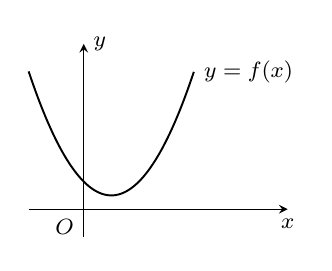
\begin{tikzpicture}[smooth,samples=300,scale=0.7,>=stealth,font=\footnotesize]
			\draw[->] (-1,0)--(3.7,0) node[below]{$x$};
			\draw[->] (0,-0.5)--(0,3) node[right]{$y$};
			\draw (0,0) node[below left]{$O$};
			\draw[line width=0.7pt,domain=-1:2] plot(\x,{(\x)^2-\x +0.5})node[right]{$y=f(x)$};
		\end{tikzpicture}
	}
	\loigiai{
		Từ hình vẽ suy ra hệ số $a>0$ và $\Delta <0$ (vô nghiệm).
	}
\end{ex}

\begin{ex}%[0D4Y5-1]
	Bảng xét dấu nào sau đây là bảng xét dấu của biểu thức $f(x)=-x^2+14x-49$?
	\choice
	{
\begin{tikzpicture}[font=\footnotesize]
			\tkzTabInit[nocadre=false,lgt=1,espcl=1.3,deltacl=0.6]
			{$x$ /0.6,$f(x)$ /0.6}
			{$-\infty$,$7$,$+\infty$}
			\tkzTabLine{,+,$0$,+,}
	\end{tikzpicture}}
	{
\begin{tikzpicture}[font=\footnotesize]
			\tkzTabInit[nocadre=false,lgt=1,espcl=1.3,deltacl=0.6]
			{$x$ /0.6,$f(x)$ /0.6}
			{$-\infty$,$7$,$+\infty$}
			\tkzTabLine{,+,$0$,-,}
	\end{tikzpicture}}
	{\True 
\begin{tikzpicture}[font=\footnotesize]
			\tkzTabInit[nocadre=false,lgt=1,espcl=1.3,deltacl=0.6]
			{$x$ /0.6,$f(x)$ /0.6}
			{$-\infty$,$7$,$+\infty$}
			\tkzTabLine{,-,$0$,-,}
	\end{tikzpicture}}
	{
\begin{tikzpicture}[font=\footnotesize]
			\tkzTabInit[nocadre=false,lgt=1,espcl=1.3,deltacl=0.6]
			{$x$ /0.6,$f(x)$ /0.6}
			{$-\infty$,$7$,$+\infty$}
			\tkzTabLine{,-,$0$,+,}
	\end{tikzpicture}}
	\loigiai{
		Ta có $f(x)= 0 \Leftrightarrow -x^2+14x-49=0 \Leftrightarrow x=7$.\\
		Bảng xét dấu
		\begin{center}
			
\begin{tikzpicture}[font=\footnotesize]
				\tkzTabInit[nocadre=false,lgt=1.3,espcl=1.8,deltacl=0.6]
				{$x$ /0.6,$f(x)$ /0.6}
				{$-\infty$,$7$,$+\infty$}
				\tkzTabLine{,-,$0$,-,}
			\end{tikzpicture}
		\end{center}
	}
\end{ex}



\begin{ex}%[0D4B5]
	Tìm tập nghiệm của bất phương trình $-5x^2+4x+12>0$.
	\choice{$\left(-\infty;-\dfrac{6}{5}\right)\cup \left(2;+\infty\right)$}
	{$\left(-2;\dfrac{6}{5}\right)$}
	{\True $\left(-\dfrac{6}{5};2\right)$}
	{$\left(-\infty;-2\right)\cup \left(\dfrac{6}{5};+\infty\right)$}
	\loigiai{
		Đặt $f(x)=-5x^2+4x+12$.\\
		Bảng xét dấu của $f(x)$ như sau
		\begin{center}
			
\begin{tikzpicture}
				\tikzset{t style/.style = {style = draw}}
				\tkzTabInit[lgt=1.5,espcl=2]
				{$x$ /0.7, $f(x)$ /0.8}
				{$-\infty$, $-\dfrac{6}{5}$, $2$, $+\infty$}
				\tkzTabLine{ ,-,0,+,0,-, }
			\end{tikzpicture}
		\end{center}
		Suy ra tập nghiệm là $\left(-\dfrac{6}{5};2\right)$.
	}
\end{ex}
\begin{ex}%[0D4B5-2]%
	Tập xác định của hàm số $y=\sqrt{-x^2+2x+3}$ là
	\choice
	{$(1;3)$}
	{$(-\infty;-1) \cup (3;+\infty)$}
	{$(-\infty;-1] \cup [3;+\infty)$}
	{\True $[-1;3]$}
	\loigiai{
		Điều kiện xác định của hàm số là $-x^2 + 2x + 3 \geq 0 \Leftrightarrow -1 \leq x \leq 3$.\\
		Vậy tập xác định của hàm số là $\mathscr D = [-1; 3]$.}
\end{ex}
\begin{ex}%[0D4B3]
	Tập xác định của hàm số $y=\sqrt{2x^2-5x-2}$ là 
	\choice
	{$\left(-\infty ; \dfrac{1}{2}\right]$}
	{$[2;+\infty) $}
	{\True $\left(-\infty ; \dfrac{1}{2}\right] \cup  [2;+\infty) $}
	{$\left[\dfrac{1}{2};2\right]$}
	\loigiai{
		Điều kiện xác định $2x^2-5x-2\ge 0$. Giải bất phương trình này ta được $x\le \dfrac{1}{2}$ hoặc $x \ge 2$.\\
		Vậy tập xác định là $\left(-\infty ; \dfrac{1}{2}\right] \cup  [2;+\infty) $.
	}
\end{ex}
\begin{ex}%[0D4B3]
	Tam thức bậc hai $x^2-5x-6$ luôn dương khi
	\choice
	{\True $x<-1$ hoặc $x>6$}
	{$-1<x<6$}
	{$x\le -1$ hoặc $x\ge 6$}
	{$-1\le x\le 6$}
	\loigiai{
		Ta có $x^2-5x-6>0 \Leftrightarrow x<-1$ hoặc $x>6$.
	}
\end{ex}


\begin{ex}%[0D7H2-2]
	\immini[thm]{Cho hàm số $f(x)=ax^2+bx+c$ có đồ thị như hình bên. Tìm tập nghiệm của bất phương trình $ax^2+bx+c \le 0$.
		\choice
		{ $(-\infty;0)\cup (2;+\infty)$}
		{\True $[0;2]$ }
		{ $(-\infty;0]\cup [2;+\infty)$}
		{$(0;2)$}}{\hspace{1cm}
		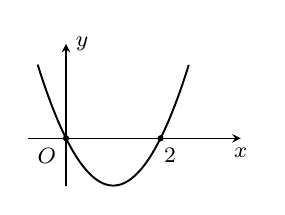
\begin{tikzpicture}[smooth,samples=300,scale=0.6,>=stealth,font=\footnotesize]
			\draw[->] (-0.8,0)--(3.7,0) node[below]{$x$};
			\draw[->] (0,-1)--(0,2) node[right]{$y$};
			\draw (0,0) node[below left]{$O$};
			\draw[line width=0.7pt,domain=-0.6:2.6] plot(\x,{(\x)^2-2*(\x)});
			\draw[fill=black] (2,0) circle(1.5pt) (0,0) circle(1.5pt);
			\node[below] at (2.2,0) {$2$};
	\end{tikzpicture}}
	\loigiai{
		$ax^2+bx+c \le 0$ tương ứng với phần đồ thị nằm phía dưới hoặc "chạm " $Ox$.\\ Từ hình vẽ, ta được $ax^2+bx+c \le 0 \Leftrightarrow 0 \le x \le 2$.
	}
\end{ex}

\begin{ex}%[0D7H2-2]
	\immini[thm]{Cho hàm số $f(x)=ax^2+bx+c$ có đồ thị như hình bên. Tìm tập nghiệm của bất phương trình $ax^2+bx+c \ge 0$.
		\choice
		{ $(-\infty;-2)\cup (1;+\infty)$}
		{ $(-\infty;-2]\cup [1;+\infty)$}
		{\True $[-2;1]$ }
		{$(0;2)$}}{\hspace{1cm}
		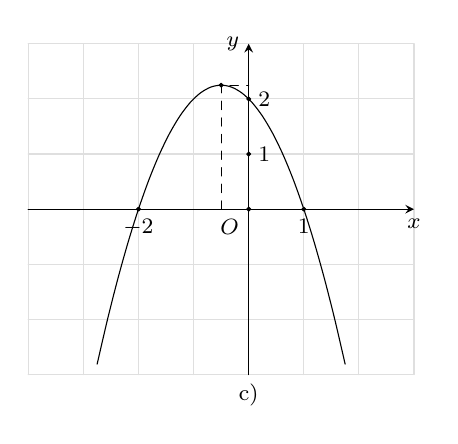
\begin{tikzpicture}[scale=.7, font=\footnotesize, line join=round, line cap=round, >=stealth]
			\draw[gray!50,opacity=.5](-4,-3)grid(3,3);
			\draw[->](-4,0)--(0,0)node[below left]{$O$}--(3,0)node[below]{$x$};
			\draw[->](0,-3)--(0,3)node[left]{$y$};
			\draw[smooth,domain=-2.75:1.75]plot(\x,{-(\x)^2-(\x)+2});
			\draw (0,-3)node[below]{c)};
			\draw(0,1)node[right]{$1$};
			\draw(0,2)node[right]{$2$};
			\draw(-2,0)node[below]{$-2$};
			\draw(1,0)node[below]{$1$};
			\draw[dashed](-0.5,0)--(-1/2,2.25)--(0,2.25);
			\foreach \x in {-2,0,1}\draw[fill](\x,0)circle(1pt);
			\foreach \x in {1,2}\draw[fill](0,\x)circle(1pt);
			\draw[fill](-1/2,2.25)circle(1pt);
			
	\end{tikzpicture}}
	\loigiai{
		$ax^2+bx+c \le 0$ tương ứng với phần đồ thị nằm phía trên hoặc "chạm " $Ox$.\\ Từ hình vẽ, ta được $ax^2+bx+c \ge 0 \Leftrightarrow -2 \le x \le 1$.
	}
\end{ex}



\begin{ex}%[0D4K5]
	Có tất cả bao nhiêu giá trị nguyên của tham số $m$ để tam thức bậc hai $f(x)=-2x^2-\left(m+2\right)x+m^2-m-1$ luôn âm trên $\mathbb{R}$?
	\choice
	{$4$}
	{$3$}
	{$2$}
	{\True $1$}
	\loigiai{
		Tam thức bậc hai $f(x)$ có $a=-2<0$ nên 
		\begin{eqnarray*}
			\allowdisplaybreaks
			f(x)<0,\, \forall x \in \mathbb{R}
			&\Leftrightarrow&\Delta <0 \Leftrightarrow (m+2)^2+8(m^2-m-1)<0\\
			&\Leftrightarrow& 9m^2-4m-4<0 \\
			&\Leftrightarrow& \dfrac{2-2\sqrt{10}}{9}<m<\dfrac{2+2\sqrt{10}}{9}
		\end{eqnarray*}
		Các số nguyên thỏa điều kiện trên là $m=0$.
	}
\end{ex}

\begin{ex}%[0D4K5-2]
	Tìm tất cả giá trị thực của tham số $m$ để $-2x^2+(m+2)x+m-4 <0$ với mọi $x \in \mathbb{R}$. 
	\choice
	{$m<-14$ hoặc $m>2$}
	{$-14\le m\le 2$}
	{$-2<m<14$}
	{\True $-14<m<2$}
	\loigiai
	{
		Tam thức $f(x)$ có $a=-2<0$. Do đó
		\allowdisplaybreaks
		\begin{eqnarray*}
			f(x)<0,\forall x \Leftrightarrow (m+2)^2+8(m-4)<0 \Leftrightarrow m^2+12m-28\leq 0 \Leftrightarrow -14<m<2.
		\end{eqnarray*}
		Vậy $-14<m<2$ là các giá trị cần tìm.
	}
\end{ex}

\begin{ex}
	Lợi nhuận thu được từ việc sản xuất và bán $x$ sản phẩm thủ công của một cửa hàng là 
	$I(x)=-0{,}1x^2+235x-70000$ với $I$ được tính bằng nghìn đồng. Hỏi số lượng sản phẩm bán ra tối thiểu là bao nhiêu thì cửa hàng có lãi?
	\choice
	{$300$}
	{$250$}
	{\True $350$}
	{$320$}
	\loigiai{
		Cửa hàng có lãi khi và chỉ khi $I(x)>0$ hay $-0{,}1x^2+235x-70000>0$, tức là $350<x<2000$.\\
		Vậy khi sản xuất và bán ra từ $351$ đến $1999$ sản phẩm thì cửa hàng có lãi.}
\end{ex}


\begin{ex}%[0D4T5-2]
	\immini[thm]{Xét một hình vuông lớn có kích thước $20 \times 20$. Từ hình vuông lớn, người ta cắt ra một hình vuông nhỏ như hình bên (\textit{các đỉnh hình vuông nhỏ nằm trên cạnh hình vuông lớn}). Tìm tập hợp các giá trị của $x$ để diện tích hình vuông nhỏ không vượt quá $208$.
		\choice
		{\True $8 \leq x \leq 12$}
		{$6 \leq x \leq 14$}
		{$12 \leq x \leq 14$}
		{$12 \leq x \leq 18$}	
	}{\hspace{1cm}\begin{tikzpicture}[scale=1, line join = round, line cap = round]
			\tikzset{label style/.style={font=\footnotesize}}
			\tkzDefPoints{0/0/B,2/2/O}
			\tkzDefPointBy[rotation=center O angle -90](B)
			\tkzGetPoint{A}
			\tkzDefPointBy[rotation=center O angle 180](B)
			\tkzGetPoint{D}
			\tkzDefPointBy[rotation=center O angle 90](B)
			\tkzGetPoint{C}
			\tkzDefPointBy[homothety=center A ratio 0.3](D)
			\tkzGetPoint{E}
			\tkzDefPointBy[rotation=center O angle -90](E)
			\tkzGetPoint{F}
			\tkzDefPointBy[rotation=center O angle 180](E)
			\tkzGetPoint{G}
			\tkzDefPointBy[rotation=center O angle 90](E)
			\tkzGetPoint{H}
			\tkzDrawPolygon[color=black](A,B,C,D)
			\tkzDrawPolygon[color=magenta](E,F,G,H)
			\tkzDefPointBy[homothety=center B ratio 1.05](A)
			\tkzGetPoint{M}
			\tkzDefPointBy[homothety=center B ratio 1.05](C)
			\tkzGetPoint{P}
			\tkzDefPointBy[translation=from A to E](M)
			\tkzGetPoint{N}
			\tkzDefPointBy[translation=from C to D](P)
			\tkzGetPoint{Q}
			\tkzFillPolygon[pattern=dots,pattern color=green](E,F,G,H)
			\tkzDrawSegments[<->,above](M,N P,Q)
			\tkzLabelSegment[above](M,N){$x\;\mathrm{cm}$}
			\tkzLabelSegment[right](P,Q){$20\;\mathrm{cm}$}
			%\tkzMarkAngle[mark=|](C,A,B)
	\end{tikzpicture}}
	\loigiai{
		\immini{Gọi $E,F,G,H$ là bốn đỉnh của viên gạch hình vuông nội tiếp trong hình vuông $ABCD$ có cạnh $20$ cm như hình vẽ\\
			Ta có cạnh viên gạch là 
			$$EF=\sqrt{x^2+(20-x)^2}=\sqrt{2x^2-40x+400}.$$
			Diện tích của viên gạch là $EF^2=2x^2-40x+400$.
		}
		{\hspace{1cm}\begin{tikzpicture}[scale=1, line join = round, line cap = round]
				\path (0,0) coordinate (B)
				(2,2) coordinate (O)
				($(O)!1!-90:(B)$) coordinate (A)
				($(O)!1!180:(B)$) coordinate (D)
				($(O)!1!90:(B)$) coordinate (C)
				($(A)!0.3!(D)$) coordinate (E)
				($(O)!1!-90:(E)$) coordinate (F)
				($(O)!1!180:(E)$) coordinate (G)
				($(O)!1!90:(E)$) coordinate (H)
				($(B)!1.05!(A)$) coordinate (M)
				($(B)!1.05!(C)$) coordinate (P)
				($(E)+(M)-(A)$) coordinate (N)
				($(P)+(D)-(C)$) coordinate (Q)
				;
				\draw (A)--(B)--(C)--(D)--cycle;
				\fill[color=blue] (E)--(F)--(G)--(H)--cycle;
				\fill[color=red,opacity=0.3] (A)--(B)--(C)--(D)--cycle;
				
				\tkzLabelSegment[above](A,E){$x$}
				\tkzLabelSegment[above](E,D){$20-x$}
				\foreach \x/\goc in {A/180,B/180,C/10,D/80,E/90,F/10,G/-90,H/180}
				\draw[fill=black] (\x) node[shift={(\goc:7pt)}]{$\x$} circle (1pt);
			\end{tikzpicture}
		}\noindent
		Theo đề ta có diện tích viên gạch không vượt quá $208$ cm$^2$, suy ra
		$$2x^2-40x+400 \leq 208 \Leftrightarrow 2x^2-40x+192 \leq 0
		\Leftrightarrow 8 \leq x \leq 12.$$
	}
\end{ex}


\ind{PHẦN II.} \inden{Câu trắc nghiệm đúng sai. Trong mỗi ý a), b), c), d) ở mỗi câu, học sinh chọn đúng hoặc sai.}
\setcounter{ex}{0}
\begin{ex}%[0D4B5-1]
	Cho hàm số bậc hai $y=f(x)$ có bảng biến thiên như hình bên dưới:
	\begin{center}
		
\begin{tikzpicture}
			\tikzset{t style/.style = {style = draw}}
			\tkzTabInit[lgt=1.5,espcl=2]
			{$x$ /0.7, $f(x)$ /0.8}
			{$-\infty$, $-2$, $4$, $+\infty$}
			\tkzTabLine{ ,-,0,+,0,-, }
		\end{tikzpicture}
	\end{center}
	Xét tính đúng sai của các khẳng định sau:
	\choiceTF
	{$f(-1)<0$}
	{$f(5)>0$}
	{\True Tập nghiệm của bất phương trình $f(x) \le 0$ là $[-2;3]$}
	{Tập nghiệm của bất phương trình $f(x) < 0$ là $(-\infty;-2)$}
	\loigiai{
		Từ bảng xét dầu, suy ra
		\begin{itemchoice}
			\itemch $f(-1)>0$, do $-1 \in (-2;4)$.
			\itemch $f(5)<0$, do $5 \in (4,+\infty)$.
			\itemch Tập nghiệm của bất phương trình $f(x) \le 0$ là $[-2;3]$.
			\itemch Tập nghiệm của bất phương trình $f(x) < 0$ là $(-\infty;-2) \cup (4;\infty)$
		\end{itemchoice}
	}
\end{ex}

\begin{ex}%[0D7H2-2]
	\immini[thm]{Cho hàm số $f(x)=ax^2+bx+c$ có đồ thị như hình bên. Xét tính đúng sai của các khẳng định sau:
		\choiceTF
		{Hệ số $a<0$}
		{\True Tập nghiệm của bất phương trình $f(x) \ge  0$ là $[0;4]$}
		{Tập nghiệm của bất phương trình $f(x) \ge 4$ là $\varnothing $}
		{\True Tập nghiệm của bất phương trình $f(x) \ge  3$ là $[1;3]$}
	}{\hspace{1cm}
		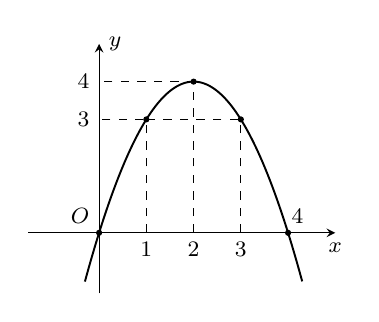
\begin{tikzpicture}[smooth,samples=300,scale=0.6,y=0.8cm,>=stealth,font=\footnotesize]
			\draw[->] (-1.5,0)--(5,0) node[below]{$x$};
			\draw[->] (0,-1.6)--(0,5) node[right]{$y$};
			\draw (0,0) node[above left]{$O$};
			\draw[line width=0.7pt,domain=-0.3:4.3] plot(\x,{-(\x)^2+4*(\x)});
			\draw[fill=black] (4,0) circle(1.5pt) (0,0) circle(1.5pt) (2,4) circle(1.5pt) (1,3) circle(1.5pt) (3,3) circle(1.5pt);
			\draw[dashed] (2,0)node[below]{$2$}--(2,4)--(0,4)node[left]{$4$}
			(1,0)node[below]{$1$}--(1,3)--(0,3)node[left]{$3$}
			(3,0)node[below]{$3$}--(3,3)--(1,3);
			\node[above] at (4.2,0) {$4$};
	\end{tikzpicture}}
	\loigiai{
	}
\end{ex}

\begin{ex}%[0D7V2-3]
	Cho $f(x)$, $g(x)$ là các hàm số xác định trên $\mathbb{R}$, có bảng xét dấu như sau
	\begin{center}
		
\begin{tikzpicture}
			\tkzTabInit[nocadre=false,lgt=1.5,espcl=2.5,deltacl=0.6] %phần bắt buộc
			{$x$/0.6, $f(x)$/0.6, $g(x)$/0.6} %phần bắt buộc
			{$-\infty$, $1$, $2$, $3$, $+\infty$} % hàng 1 cột 2
			\tkzTabLine{,+,z,-,t,-,z,+,}
			\tkzTabLine{,-,t,-,z,+,t,+,}
		\end{tikzpicture}
	\end{center}
	Xét tính đúng sai của các khẳng định sau:
	\choiceTF
	{Tập nghiệm của bất phương trình $f(x)< 0$ là $(1;2)\cup (2;3)$}
	{\True Tập nghiệm của bất phương trình $g(x) \geq 0$ là $[2;+\infty)$}
	{\True Tập nghiệm của bất phương trình $f(x) \cdot g(x) \le 0$ là $(-\infty;1]\cup [2;3]$}
	{Tập nghiệm của bất phương trình $\dfrac{f(x)}{g(x)}\geq 0$ là $[1;2]\cup [3;+\infty)$}
	\loigiai
	{
	}
\end{ex}

\begin{ex}%[0D7V2-7]
	Người ta thử nghiệm ném một quả bóng trên Mặt Trăng. Nếu quả bóng được ném lên từ độ cao $h_0$ (m) so với bề mặt của Mặt Trăng với vận tốc $v_0$ (m/s) thì độ cao của bóng sau $t$ giây được cho bởi hàm số $h(t)=-\dfrac{1}{2}gt^2+v_0t+h_0$ với $g=1{,}625$ (m/s$^2$) là gia tốc trọng trường của Mặt Trăng. Biết độ cao ban đầu của quả bóng vào các thời điểm $8$ giây và $12$ giây lần lượt là $30$ m và $5$ m. Xét tính đúng sai của các khẳng định sau:
	\choiceTF
	{Vận tốc ném $v_0=10$ m/s}
	{Độ cao ban đầu của quả bóng $h_0=2$ m}
	{$h(t)=-0,8125t^2+10t+2$}
	{Quả bóng ở độ cao trên $29$ m trong khoảng $3,15$ giây}
	\loigiai{
		\begin{enumerate}
			\item Ta có $h(t)=-0{,}8125t^2+v_0t+h_0$, $h(8)=30$ và $h(12)=5$.\\
			Do đó $\heva{&-52+8v_0+h_0=30\\&-117+12v_0+h_0=5}$ hay $\heva{&v_0=10\\&h_0=2.}$\\
			Vậy $h(t)=-0,8125t^2+10t+2$.
			\item Quả bóng đạt độ cao trên $29$ m khi và chỉ khi $-0{,}8125t^2+10t+2>29$, hay $4<t<8{,}31$.\\
			Vậy quả bóng ở độ cao trên $29$ m trong khoảng $8{,}31-4=4{,}31$ giây.
		\end{enumerate}
	}
\end{ex}

\ind{PHẦN III.} \inden{Câu trả lời ngắn.}
\setcounter{ex}{0}
\begin{ex}%[0D7H1-2]
	Tập nghiệm của bất phương trình $x^2-x-6\leqslant 0$ có bao nhiêu số nguyên?\\
	\par\shortans[3]{$6$}
	\loigiai{
		Ta có $x^2-x-6\leqslant 0\Leftrightarrow -2\leq x\leq 3$.\\Vậy tập nghiệm của bất phương trình đã cho là $S=[-2;3]$.
		Tập này có 6 số nguyên.
	}
\end{ex}
%%=====Câu 2
\begin{ex}%[0D7H1-2]
	Có bao nhiêu giá trị nguyên của tham số $m$ để phương trình $4x^2+2(m-2)x+m^2=0$ có nghiệm?
	\par\shortans[3]{$3$}
	\loigiai{
		Phương trình có nghiệm khi và chỉ khi 
		\[\Delta'=(m-2)^2-4m^2=-3m^2-4m+4 \geq 0 \Leftrightarrow -2 \leq m \leq \dfrac{2}{3}.\]
		Vậy $-2 \leq m \leq \dfrac{2}{3}$.\\
		Do $m \in \mathbb{Z}$ nên $m \in \{-2;-1;0\}$.
	}
\end{ex}
%%=====Câu 3
\begin{ex}%[0D7H1-5]
	Một quả bóng được ném thẳng lên từ độ cao $1{,}6 \mathrm{~m}$ so với mặt đất với vận tốc $10 \mathrm{~m} / \mathrm{s}$. Độ cao của bóng so với mặt đất (tính bằng mét) sau $t$ giây được cho bởi hàm số $h(t) = -4{,}9t^2 + 10t + 1{,}6$. Hỏi bóng ở độ cao trên $5 \mathrm{~m}$ trong khoảng thời gian bao lâu? (Kết quả tính bằng giây và làm tròn đến hàng phần trăm).\\
	\shortans[3]{$1,18$}
	\loigiai{
		Giải bất phương trình $-4{,}9t^2 + 10t + 1{,}6 > 5$.\\
		Ta kết luận được bóng ở độ cao trên $5 \mathrm{~m}$ trong thời gian khoảng 1,18 giây.
	}
\end{ex}
%%=====Câu 4
\begin{ex}%[0D7V1-5]
	Một vật được ném theo phương thẳng đứng xuống dưới từ độ cao $300 \mathrm{~m}$ với vận tốc ban đầu $v_0=10 \mathrm{~m} / \mathrm{s}$. Giả thiết rằng sức cản của không khí là không đán kể, hỏi sau ít nhất bao nhiêu giây, vật đó cách mặt đất không quá $120$ m? (làm tròn kết quả đến hàng phần trăm).
	\par\shortans[3]{$7,17$}
	\loigiai{
		Độ cao của vật so với mặt đất được cho bởi công thức
		\[h(t) = h_0 + v_0t - \dfrac{1}{2}gt^2 = 300 + 10t - 4{,}9t^2(\mathrm{~m}).\]
		Vật cách mặt đất không quá $100 \mathrm{~m}$ khi và chỉ khi 
		\allowdisplaybreaks
		\begin{eqnarray*}
			h(t) \leq 120 \Leftrightarrow 300 + 10t - 4{,}9t^2 \leq 120
			&\Leftrightarrow& 4{,}9t^2 - 10t - 180 \geq 0\\
			&\Leftrightarrow& \heva{&t \geq \dfrac{5+\sqrt{907}}{4{,}9} \\&
				t \leq \dfrac{5 - \sqrt{907}}{4{,}9}}\\
			&\Rightarrow& t \geq \dfrac{5 + \sqrt{907}}{4{,}9} \approx 7{,}17 \text{(s) (vì } t \geq 0).
		\end{eqnarray*}
		Vậy sau ít nhất $7{,}17$ (s) thì vật đó cách mặt đất không quá $120 \mathrm{~m}$.
	}
\end{ex}


\begin{ex}%[0D7V1-5]
	Một chiếc cổng có hình parabol với chiều cao $5$ m và khoảng cách giữa hai chân cổng là $4$ m. Người ta cần chuyển một thùng hàng hình hộp chữ nhật với chiều cao $3$ m. Hỏi chiều rộng của thùng hàng tối đa là bao nhiêu để thùng có thể chuyển lọt qua được cổng? (Đáp số làm tròn đến hàng phần trăm)
	\par\shortans[3]{$2{,}52$}
	\loigiai{
		\immini
		{Đặt gốc tọa độ tại một chân cổng như hình, ta viết phương trình $y=ax^2+bx+c$ của đường viền cổng.\\
			Ta có một chân cổng có tọa độ $(0; 0)$ nên ta có $c=0$.\quad(1)\\
			Ta có một chân cổng có tọa độ $(4; 0)$ nên ta có \\$16a+4b+c=0$. \quad(2)\\
			Ta có đỉnh cổng có tọa độ $(2; 5)$ nên ta có \\$4a+2b+c=5$.\quad(3)\\
			Thay (1) vào (2) và (3) ta có hệ phương trình $\heva{&16a+4b=0\\&4a+2b=5.}$\\
			Do đó $a=-1{,}25$, $b=5$ và $c=0$.
		}
		{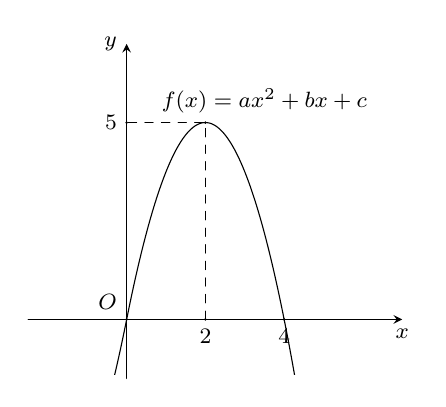
\begin{tikzpicture}[scale=0.5, font=\footnotesize, line join=round, line cap=round, >=stealth]
				\def\xmin{-2.5} \def\xmax{7}
				\def\ymin{-1.5} \def\ymax{7} 
				\draw[->] (\xmin,0)--(\xmax,0) node [below]{$x$};
				\draw[->] (0,\ymin)--(0,\ymax) node [left]{$y$};
				\fill (0,0)circle(1pt)node[above left]{$O$} (2,0)circle(1pt)node[below]{$2$} (4,0)circle(1pt)node[below]{$4$}
				(0,5)circle(1pt)node[left]{$5$}
				(2,5)circle(1pt);
				\draw (3.5,5)node[above]{$f(x)=ax^2+bx+c$};
				\draw[dashed] (2,0)--(2,5)--(0,5);
				\clip (\xmin+0.1,\ymin+0.1) rectangle (\xmax-0.1,\ymax-0.1);
				\draw[smooth,samples=300] plot(\x,{-1.25*\x^2+5*\x});
			\end{tikzpicture}
		}\noindent
		Vậy phương trình của vòm cổng là $y = -1{,}25x^2 + 5x$.\\
		Ta xác định các hoành độ $x$ mà tại đó vòm cổng cao hơn thùng hàng bằng cách giải bất phương trình $y= -1{,}25x^2 + 5x \geq 3$.\\
		Ta có $-1{,}25x^2 + 3{,}2x \geq 3$ khi và chỉ khi $0{,}74 \leq x \leq 3{,}26$.\\
		Vậy chiều rộng tối đa của thùng hàng là $3{,}26 - 0{,}74 = 2{,}52$ m.
	}
\end{ex}


%%=====Câu 6
\begin{ex}%[0D7V1-5]
	Tổng chi phí $T$ (đơn vị tính: nghìn đồng) để sản xuất $Q$ sản phẩm được cho bởi biểu thức $T=Q^2+30Q+3300$; giá bán của 1 sản phẩm là $170$ nghìn đồng. Số sản phẩm được sản xuất trong khoảng nào để đảm bảo không bị lỗ (giả thiết các sản phẩm được bán hết)?
	\par\shortans[]{1,41}
	\loigiai{
		Để đảm bảo không bị lỗ thì $T=Q^2+30Q+3300 \le 170Q \Leftrightarrow Q^2-140Q+3300\le 0$.\\
		Tam thức bậc hai $Q^2-140Q+3300$ có hai nghiệm $x_1=110, x_2=30$ và có hệ số $a=1>0$.\\
		Sử dụng định lí về dấu của tam thức bậc hai, ta thấy tập hợp những giá trị của $x$ sao cho tam thức $Q^2-140Q+3300\le 0$ là $\left(30;110\right)$.\\
		Vậy số sản phẩm được sản xuất trong khoảng $\left(30;110\right)$ để đảm bảo không bị lỗ.
	}
\end{ex}

\ind{PHẦN IV.} \inden{Tự luận.}
\setcounter{ex}{0}
\begin{ex}%[0D7H2-1]
	Giải các bất phương trình sau:
	\begin{enumEX}[a)]{2}
		\item  $x^2-3x+2<0$ 
		\item  $6x^2+x-1 \le 0$
		\item $-9x^2 + 6x -1>0$.
		\item $12-x-x^2\ge 0$.
	\end{enumEX}
	\loigiai{
		\begin{enumerate}[a)]
			\item Đặt $f(x)=x^2-3x+2$ và $f(x)=0\Leftrightarrow x^2-3x+2=0\Leftrightarrow\hoac{&x=2\\&x=1.}$\\
			Bảng xét dấu
			\begin{center}
				
\begin{tikzpicture}[>=stealth]
					\tkzTabInit[nocadre=false,lgt=1.2,espcl=2,deltacl=1]{$x$/.7 ,$f(x)$/.7}
					{$-\infty$ , $1$ , $2$ , $+\infty$}
					\tkzTabLine{ ,+ , $0$ , - , $0$ , + , }
				\end{tikzpicture}
			\end{center}
			Dựa vào bảng xét dấu, tập nghiệm của bất phương trình đã cho là
			\[S=(1;2).\]
			\item Bảng xét dấu
			\begin{center}
				
\begin{tikzpicture}[>=stealth]
					\tkzTabInit[nocadre=false,lgt=3,espcl=2,deltacl=1]{$x$/1 ,$6x^2+x-1$/.7}
					{$-\infty$ , $-\dfrac{1}{2}$ , $\dfrac{1}{3}$ , $+\infty$}
					\tkzTabLine{ ,+ , $0$ , - , $0$ ,+ , }
				\end{tikzpicture}
			\end{center}
			Từ bảng xét dấu, ta có tập nghiệm của bất phương trình là
			\[S=\left[-\dfrac{1}{2};\dfrac{1}{3}\right].\]
			\item Cho $-9x^2 + 6x -1=0 \Leftrightarrow x = \dfrac{1}{3}$.
			Bảng xét dấu
			\begin{center}
				
\begin{tikzpicture}
					\tkzTabInit
					[lgt=2.8,espcl=2] % tùy chọn
					{$x$/1, $-9x^2 + 6x -1 $/1.5} % cột 1
					{$-\infty $, $\dfrac{1}{3}$ ,$+ \infty $} % hàng 1 cột 2
					\tkzTabLine{, -, z , -, } % hàng 2 cột 2
				\end{tikzpicture}
			\end{center}
			Vậy $S= \emptyset$.
			\item Cho $-x^2 -x+12=0 \Leftrightarrow \hoac{&x =-4 \\& x=3.}$\\
			Bảng xét dấu
			\begin{center}
				
\begin{tikzpicture}
					\tkzTabInit
					[lgt=2.5,espcl=2] % tùy chọn
					{$x$/1, $-x^2 -x+12 $/1.5} % cột 1
					{$-\infty $, $-4$,$3$ ,$+ \infty $} % hàng 1 cột 2
					\tkzTabLine{, - , z , + , z , -, } % hàng 2 cột 2
				\end{tikzpicture}
			\end{center}
			Vậy $S= [-4;3]$.
	\end{enumerate}}
\end{ex}

%%=====Bài 2
\begin{ex}%[0D4B5-2]
	Tìm tất cả giá trị thực của tham số $m$ để
	\begin{enumEX}[a)]{1}
		\item phương trình $2x^2+2\left( m+2 \right)x+3+4m+{m^2}=0$ có nghiệm.
		\item phương trình $x^2-(m+1)x+1=0$ vô nghiệm.
		\item phương trình $x^2+2(m+1)x+9m-5=0$ có hai nghiệm phân biêt.
	\end{enumEX}
	\loigiai
	{\begin{enumerate}[a)]
			\item Phương trình $2x^2+2(m+2)x+3+4m+m^2=0$ có $\Delta'=(m+2)^2-2(m^2+4m+3) = -m^2-4m-2$.\\
			Yêu cầu bài toán thỏa mãn khi
			\allowdisplaybreaks
			\begin{eqnarray*}
				\Delta' \geq 0 &\Leftrightarrow & -m^2-4m-2 \geq 0\\
				&\Leftrightarrow & -2-\sqrt{2} \leq m \leq -2+\sqrt{2}.
			\end{eqnarray*}
			Vậy với $m \in \left[-2-\sqrt{2};-2+\sqrt{2}\right]$ thì phương trình đã cho có nghiệm.
			\item Phương trình vô nghiệm khi và chỉ khi
			\begin{eqnarray*}
				\Delta <0 \Leftrightarrow (m+1)^2-4<0 \Leftrightarrow m^2+2m-3<0 \Leftrightarrow -3<m<1.
			\end{eqnarray*}
			Vậy $-3<m<1$ là các giá trị thỏa mãn yêu cầu bài toán.
			\item Phương trình có hai nghiệm phân biệt khi và chỉ khi
			$$\Delta=(m+1)^2-(9m-5)>0 \Leftrightarrow m^2-7m+6>0 \Leftrightarrow m<1 \text{ hoặc } m>6.$$
		\end{enumerate}
	}
\end{ex}
%%=====Bài 3
\begin{ex}%[0D7V2-6]
	Tìm tất cả các giá trị của tham số $m$  để 
	\begin{enumEX}[a)]{1}
		\item $x^2-mx-m\ge 0$, $\forall x \in \mathbb{R}$.
		\item $-x^2+(2m-1)x+m<0$, $\forall x \in \mathbb{R}$.
		\item $(m+2)x^2+2(m+2)x+m+3 \ge 0$, $\forall x \in \mathbb{R}$.
		\item $(3m+1)x^2-(3m+1)x+m+4\geq 0$, $\forall x \in \mathbb{R}$.
	\end{enumEX}
	\loigiai{
		\begin{enumerate}[a)]
			\item Tam thức $f(x)=x^2-mx-m$ có hệ số $a=1>0$. Do đó bất phương trình $f(x) \ge 0$ nghiệm đúng với mọi $\forall x \in\mathbb{R}$ khi và chỉ khi 
			\begin{eqnarray*}
				m^2+4m\leq 0\Leftrightarrow -4\leq m\leq 0.
			\end{eqnarray*}
			Vậy $-4\le m\le 0$ là các giá trị cần tìm.
			\item Tam thức $f(x)=-x^2+(2m-1)x+m$ có hệ số $a=-1<0$ nên bất phương trình $f(x)<0$ có tập nghiệm là $\mathbb{R}$ khi
			\begin{eqnarray*}
				(2m-1)^2+4m<0 \Leftrightarrow 4m^2+1<0, \text{vô nghiệm}.
			\end{eqnarray*}
			Vậy không có giá trị của $m$ thỏa mãn yêu cầu bài toán.
			\item 	{\bf Trường hợp 1.} Với $m=-2$, ta được $f(x)=1>0$, luôn đúng với mọi $x$. Do đó $m=-2$ thỏa mãn yêu cầu bài toán.\\
			{\bf Trường hợp 2.} Với $m\neq -2$, yêu cầu bài toán thỏa mãn khi
			\allowdisplaybreaks
			\begin{eqnarray*}
				\heva{&m+2>0 \\&(m+2)^2-(m+2)(m+3) \leq 0} \Leftrightarrow \heva{&m>-2 \\&-m-2\leq 0} \Leftrightarrow m>-2.
			\end{eqnarray*}
			Kết hợp hai trường hợp ta được $m\ge -2$ là các giá trị cần tìm.
			\item  Xét bất phương trình $\left( 3m+1 \right)x^2-\left( 3m+1 \right)x+m+4\ge 0$.\hfill $(*)$\\
			{\bf Trường hợp 1.} Với $3m+1=0$ hay $m=-\dfrac{1}{3}$, bất phương trình $(*)$ trở thành $4-\dfrac{1}{3}\ge 0$ (luôn đúng). Do đó $m=-\dfrac{1}{3}$ là giá trị thỏa mãn yêu cầu bài toán.\\
			{\bf Trường hợp 2.} Với $3m+1\ne 0$ hay $m\ne -\dfrac{1}{3}$, bất phương trình $(*)$ nghiệm đúng với mọi $x$ khi
			\allowdisplaybreaks
			\begin{eqnarray*}
				\heva{&3m+1>0 \\&(3m+1)^2-4(3m+1)(m+4) \leq 0} \Leftrightarrow \heva{&m>-\dfrac{1}{3} \\&3m^2+46m+15 \geq 0} \Leftrightarrow \heva{&m>-\dfrac{1}{3} \\&\hoac{&m<-15 \\&m>-\dfrac{1}{3}}} \Leftrightarrow m>-\dfrac{1}{3}.
			\end{eqnarray*}
			Kết hợp hai trường hợp, ta được $m\ge -\dfrac{1}{3}$ là các giá trị cần tìm.
		\end{enumerate}
	}
\end{ex}
%%=====Bài 4
\begin{ex}%[0D3V2-6]
	\immini{Một tình huống trong huấn luyện pháo binh được mô tả như sau: Trong mặt phẳng tọa độ $Oxy$, khẩu đại bác được biểu thị bằng điểm $O(0; 0)$ và bia mục tiêu được biểu thị bằng đoạn thẳng $MN$ với $M(2100; 25)$ và $N(2100; 15)$ (Hình 29). Xạ thủ cần xác định parabol $y=-a^2x^2+10ax$ $(a>0)$ mô tả quỹ đạo chuyển động của viên đạn sao cho viên đạn bắn ra từ khẩu đại bác phải chạm vào bia mục tiêu. Tìm giá trị lớn nhất của $a$ để xạ thủ đạt được mục đích trên.
	}{\begin{tikzpicture}[scale=1, font=\footnotesize, line join=round, line cap=round, >=stealth]
			\def\a{-.25} \def\b{1} \def\c{0} % Hệ số
			\def\xt{-1} \def\xp{6} \def\yt{3} \def\yd{-1} % x_trái, x_phải, y_trên, y_dưới (giới hạn)
			\draw[->] (\xt,0)--(\xp,0) node [below]{$x$};
			\draw[->] (0,\yd)--(0,\yt) node [left]{$y$};
			\node at (0,0) [below left]{$O$};
			\clip (\xt-0.1,\yd+0.1) rectangle (\xp-0.1,\yt-0.1);
			\draw[smooth,samples=300,domain=0:4] plot(\x,{\a*(\x)^2+\b*(\x)+\c});
			\draw[fill=black] (3,0) node[shift={(-90:.4)}]{$2\,100$} circle(1pt);
			\draw[fill=black] (3,1) node[shift={(90:.4)}]{$M$} circle(1pt);
			\draw[fill=black] (3,.5) node[shift={(180:.3)}]{$N$} circle(1pt);
			\draw[line width=2pt] (3,1)--(3,.5);
			\draw (2,1) node[shift={(90:1)}]{$y=-a^2x^2+10ax$};
			\draw (2,-1) node[shift={(-90:.4)}]{Hình 29};
		\end{tikzpicture}
	}
	\loigiai{Tại vị trí $x=2\,100$, độ cao của viên đạn là
		\[y=-a^2\cdot 2\,100^2+10a\cdot 2\,100=-4\,410\,000a^2+21\,000a.\]
		Viên đạn chạm được vào bia mục tiêu khi và chỉ khi $a$ thoả mãn các bất phương trình sau
		\allowdisplaybreaks
		\begin{align*}
			&2\,100\leq\dfrac{10}{a} \tag{5}; \\
			&-4\,410\,000a^2+21\,000a\leq 25  \tag{6};\\
			&-4\,410\,000a^2+2\,1000a\geq 15  \tag{7}.
		\end{align*}
		\begin{itemize}
			\item $(5)\Leftrightarrow\dfrac{1}{a}\geq 210\Leftrightarrow a\leq\dfrac{1}{210}$. Vì $a>0$ nên $a\in\left(0;\dfrac{1}{210}\right]$.
			\item $(6) \Leftrightarrow 4\,410\,000a^2-21\,000a+25\geq 0 \Leftrightarrow(2\,100a-5)^2\geq 0$. Bất phương trình này đúng $\forall a>0$.
			\item \allowdisplaybreaks
			$\begin{aligned}[t]
				(7)&\Leftrightarrow 4\,410\,000a^2-21\,000a+15\leq 0\Leftrightarrow\dfrac{1}{420}-\dfrac{\sqrt{10}}{2\,100}\leq a\leq\dfrac{1}{420}+\dfrac{\sqrt{10}}{2\,100}\\
				&\Leftrightarrow a\in\left[\dfrac{1}{420}-\dfrac{\sqrt{10}}{2\,100};\dfrac{1}{420}+\dfrac{\sqrt{10}}{2\,100}\right].
			\end{aligned}$
		\end{itemize}
		Do $\dfrac{1}{420}-\dfrac{\sqrt{10}}{2\,100}>0$ và $\dfrac{1}{420}+\dfrac{\sqrt{10}}{2\,100}<\dfrac{1}{210}$ nên
		\[\left(0;\dfrac{1}{210}\right]\cap\left[\dfrac{1}{420}-\dfrac{\sqrt{10}}{2\,100};\dfrac{1}{420}+\dfrac{\sqrt{10}}{2\,100}\right]=\left[\dfrac{1}{420}-\dfrac{\sqrt{10}}{2\,100};\dfrac{1}{420}+\dfrac{\sqrt{10}}{2\,100}\right].\]
		Vì thế, viên đạn chạm được vào bia mục tiêu khi và chỉ khi
		\[a\in\left[\dfrac{1}{420}-\dfrac{\sqrt{10}}{2\,100};\dfrac{1}{420}+\dfrac{\sqrt{10}}{2\,100}\right].\]
		Vậy giá trị lớn nhất của $a$ là $\dfrac{1}{420}+\dfrac{\sqrt{10}}{2\,100}$.
	}
\end{ex}

%%=====Bài 5
\begin{ex}%[0D3V2-6]
	Bác Dũng muốn uốn tấm tôn phẳng có dạng hình chữ nhật với bề ngang $32$ cm thành một rãnh dẫn nước bằng cách chia tấm tôn đó thành ba phần rồi gấp hai bên lại theo một góc vuông (Hình bên dưới). 
	\begin{center}
		\begin{tikzpicture}[scale=0.8, font=\footnotesize, line join=round, line cap=round, >=stealth]
			\draw (0,0)--(4,0)--++(60:5)--++(180:4)--(0,0);
			\draw (1,0)--++(60:5) (3,0)--++(60:5);
			\draw[stealth-stealth,yshift=-.5cm] (0,0)--(4,0) node[midway,fill=white] {$32$ cm};
			\draw[stealth-stealth,yshift=.5cm] (60:5)--++(0:1) node[midway,fill=white] {$x$ cm};
			\draw[stealth-stealth,yshift=.5cm] ($(4,0)+(60:5)$)--++(180:1) node[midway,fill=white] {$x$ cm};
			\draw[stealth-stealth,yshift=.2cm] (60:5)--++(0:1);
			\draw[stealth-stealth,yshift=.2cm] ($(4,0)+(60:5)$)--++(180:1);
			\draw (8,0)--(10,0)--++(60:5)--++(180:2)--(8,0);
			\draw (8,0)--(8,1)--++(60:5)--++(-90:1);
			\draw (10,0)--(10,1)--++(60:5)--++(-90:1);
		\end{tikzpicture}	
	\end{center}
	Để đảm bảo kĩ thuật, diện tích mặt cắt ngang của rãnh dẫn nước phải lớn hơn hoặc bằng $120$ cm$^2$. Hỏi Bác Dũng cần làm rảnh dẫn nước có độ cao ít nhất là bao nhiêu cm để đảm bảo kĩ thuật?
	\loigiai
	{Khi chia tấm tôn đó thành ba phần rồi gấp hai bên lại theo một góc vuông như Hình 25 thì kích thước của mặt cắt ngang là $x$ (cm) và $32-2x$ (cm).\\
		Khi đó diện tích mặt cắt ngang là $(32-2x)$ (cm$^2$).\\
		Ta thấy: Diện tích mặt cắt ngang của rãnh dẫn nước lớn hơn $120$ cm$^2$ khi và chỉ khi
		\[(32-2x) x\geq 120\Leftrightarrow-2x^2+32x-120\geq 0.\]
		Tam thức $-2x^2+32x-120$ có hai nghiệm $x_1=6, x_2=10$ và hệ số $a=-2<0$. Sử dụng định lí về dấu của tam thức bậc hai, ta thấy tập hợp những giá trị của $x$ sao cho tam thức $-2x^2+32x-120$ mang dấu "+" là $(6; 10)$.\\
		Do đó tập nghiệm của bất phương trình $-2x^2+32x-120\geq 0$ là $[6; 10]$.\\
		Vậy rãnh dẫn nước phải có độ cao ít nhất là $6$ (cm).
	}
\end{ex}

%%=====Bài 6

\begin{ex}%[0D3V2-6]
	Một công ty du lịch thông báo giá tiền cho chuyến đi tham quan của một nhóm khách du lịch như sau: $50$ khách đầu tiên có giá là $300\,000$ đồng/người. Nếu có nhiều hơn $50$ người đăng kí thì cứ có thêm $1$ người, giá vé sẽ giảm $5\,000$ đồng/người cho toàn bộ hành khách.
	\begin{enumEX}[a)]{1}
		\item Gọi $x$ là số lượng khách từ người thứ $51$ trở lên của nhóm. Biểu thị doanh thu theo $x$.
		\item Số người của nhóm khách du lịch nhiều nhất là bao nhiêu thì công ty không bị lỗ? Biết rằng chi phí thực sự cho chuyến đi là $15\,080\,000$ đồng.
	\end{enumEX}
	\loigiai{
		\begin{enumEX}[a)]{1}
			\item Do $x$ là số lượng khách thứ $51$ trở lên nên $x>0$.\\
			Cứ thêm $1$ người thì giá còn $(300\,000-5\,000\cdot1)$ đồng/người cho toàn bộ hành khách.
			Thêm $x$ người thì giá còn $(300\,000-5\,000\cdot x)$ đồng/người cho toàn bộ hành khách.\\
			Doanh thu theo $x$ là $(50+x)\cdot(300\,000-5\,000\cdot x)$ đồng.
			\item Do chi phí thực sự cho chuyến đi là $15\,080\,000$ đồng nên để công ty không bị lỗ thì doanh thu phải lớn hơn hoặc bằng $15\,080\,000$ đồng
			Khi đó:
			\begin{center}
				
\begin{tikzpicture}[>=stealth]
					\tkzTabInit[nocadre=false,lgt=1,espcl=2,deltacl=0.5]{$h$/.7 ,$S'$/.7,$S$/2}
					{$0$ , $10\sqrt{3}$ , $+\infty$}
					\tkzTabLine{ , + , $0$ , - , }
					\tkzTabVar{-/$$ , +/$S\left(10\sqrt{3}\right)$ , -/$$}
				\end{tikzpicture}
			\end{center}
			$$
			\begin{aligned}
				(50+x) \cdot(300\,000-5000 x) \geq 15\,080\,000
				&\Leftrightarrow(50+x) \cdot 5\,000 \cdot(60-x) \geq 15\,080\,000 \\
				&\Leftrightarrow(x+50)(60-x) \geq 3\,016 \\
				&\Leftrightarrow-x^{2}+10 x+3\,000 \geq 3\,016 \\
				&\Leftrightarrow-x^{2}+10 x-16 \geq 0 \\
				&\Leftrightarrow 2 \leq x \leq 8.
			\end{aligned}
			$$
			Vậy số người của nhóm du khách nhiều nhất là $58$ người thì công ty không bị lỗ.
		\end{enumEX}
	}
\end{ex}



